\section{Threat Model}

\subsection{The Hijacked Agent Threat}

\begin{figure*}[t]
    \centering
    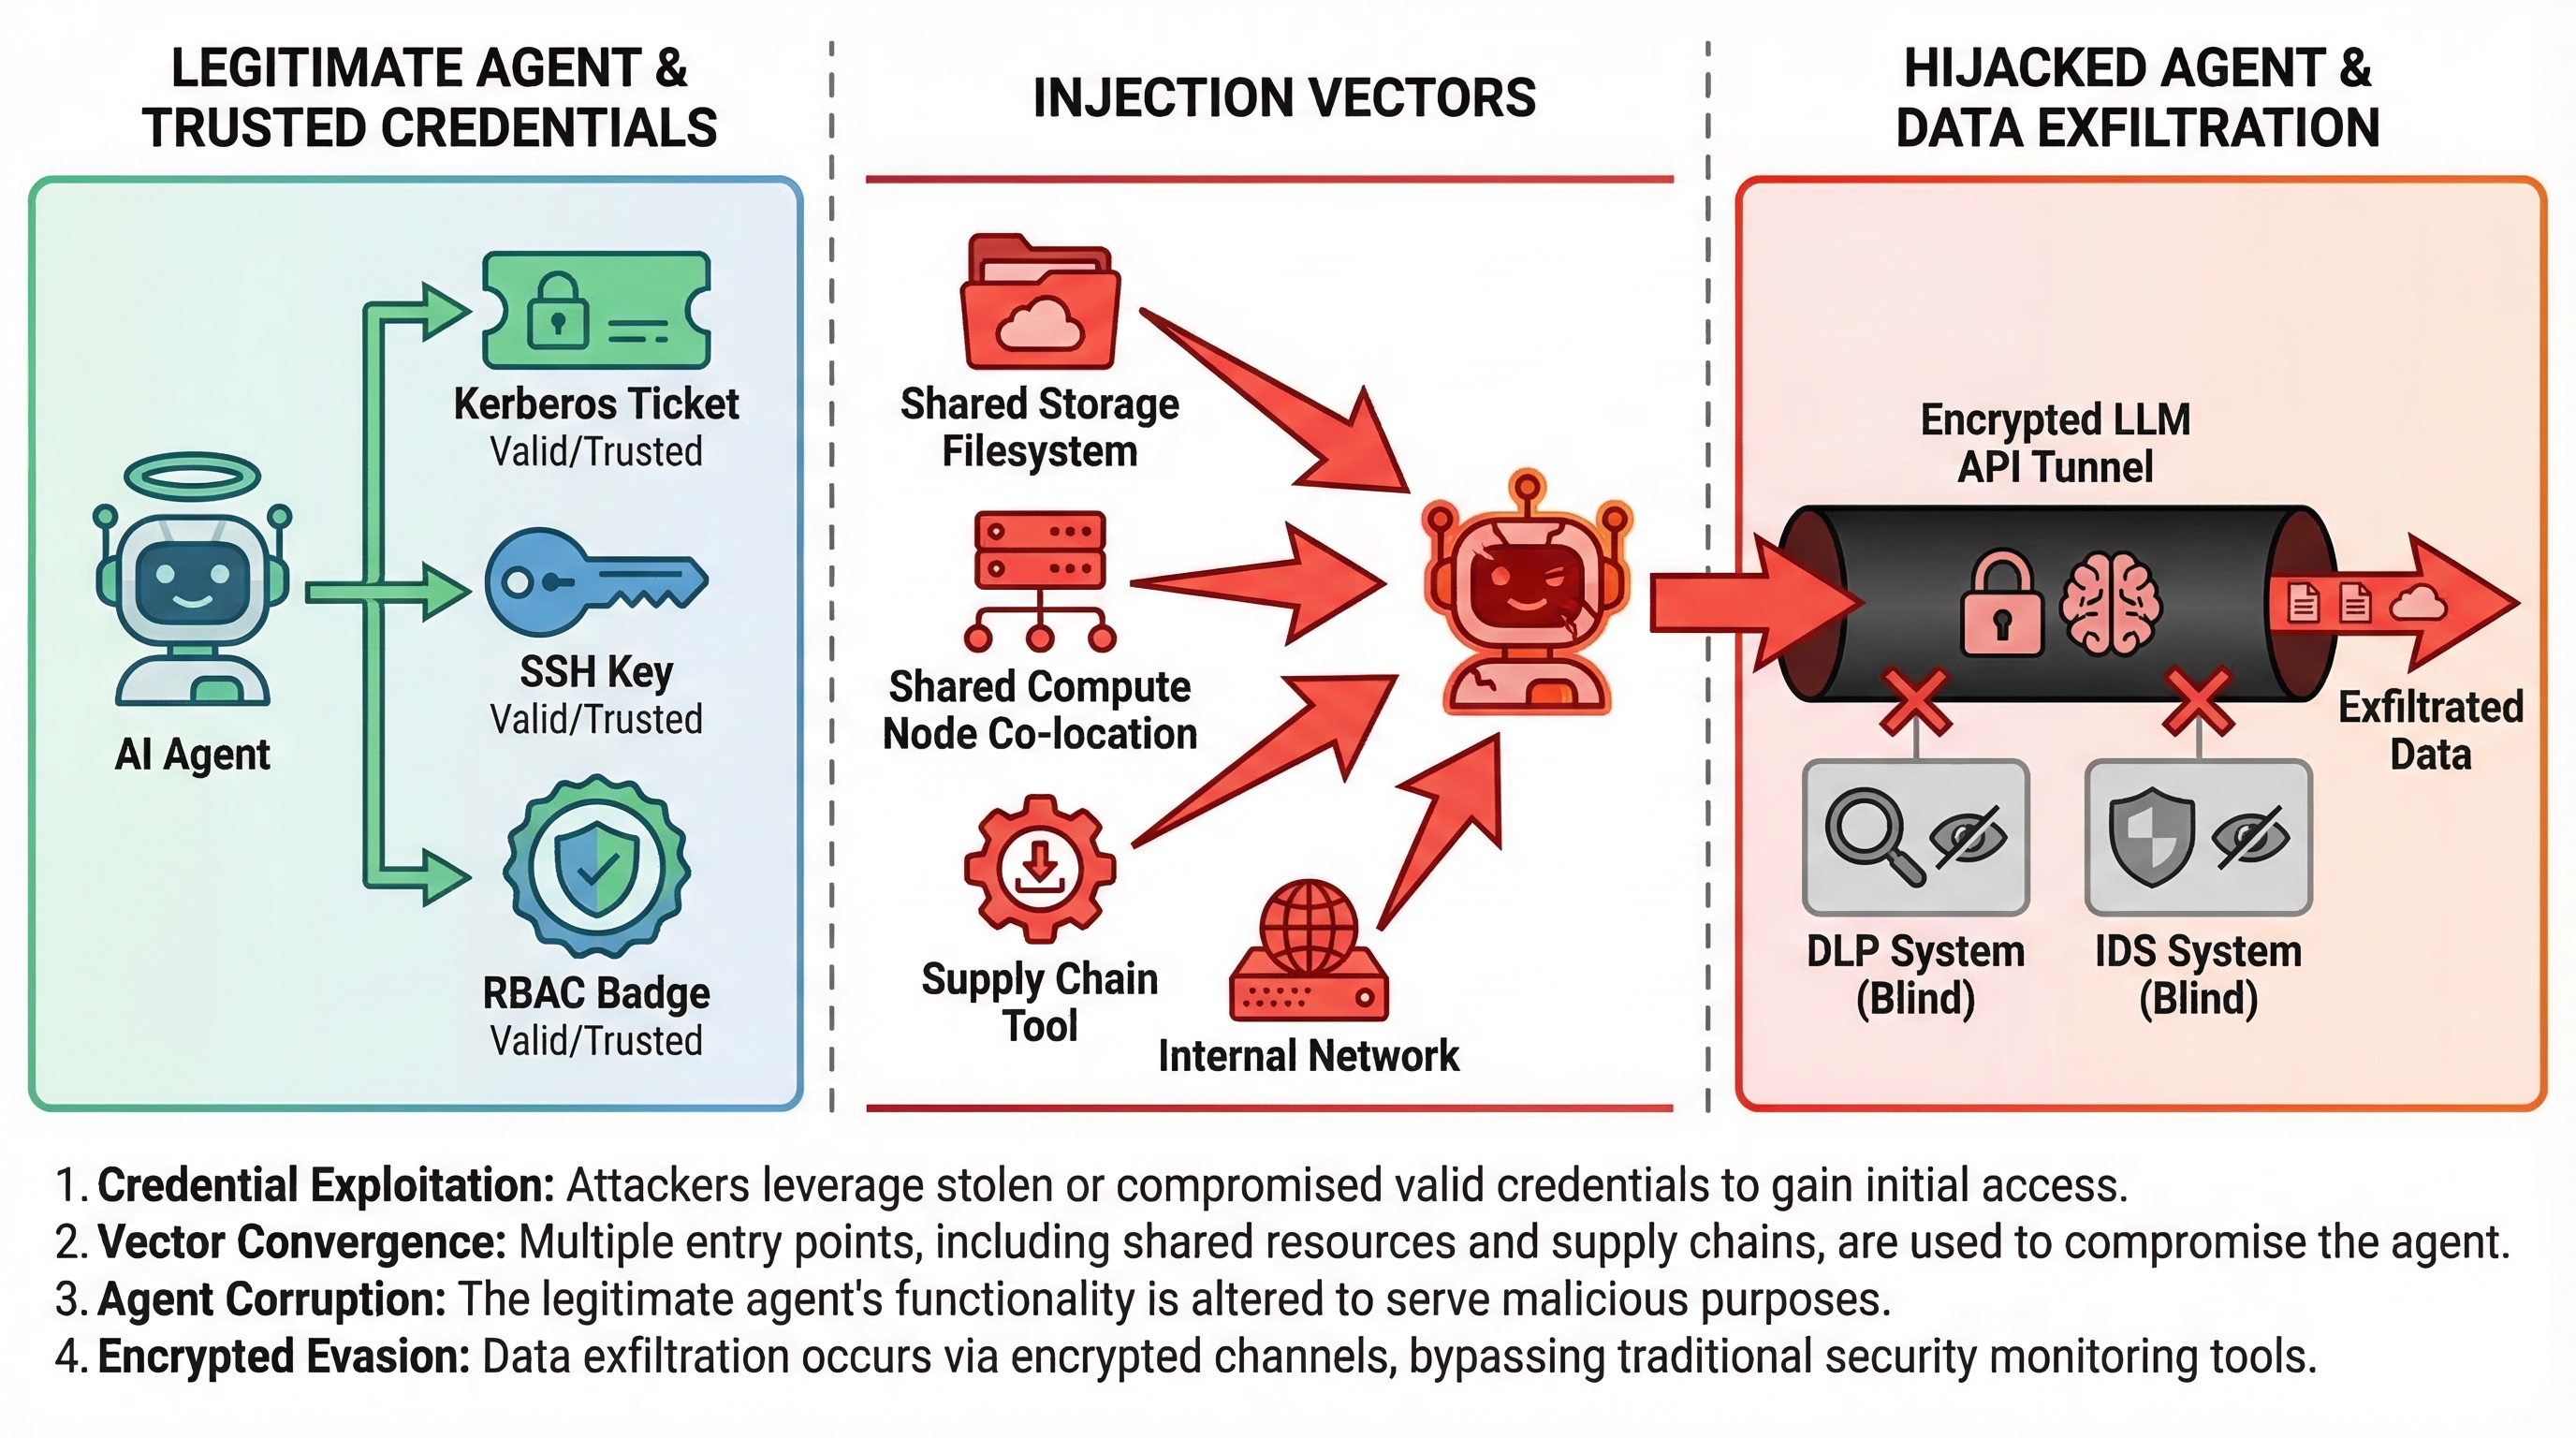
\includegraphics[width=0.94\textwidth]{../figures/threat_model.png}
    \caption{The hijacked authorized agent threat. An agent with valid credentials is subverted through injection attacks. The hijacked agent exfiltrates data through encrypted LLM API channels that are difficult for traditional DLP and perimeter monitoring to interpret.}
    \label{fig:threats}
\end{figure*}

We identify the most dangerous threat to HPC environments deploying AI agents: \textit{the hijacked authorized agent}, as illustrated in Figure~\ref{fig:threats}. Unlike malicious outsiders, which are addressed by existing authentication and authorization mechanisms, a hijacked agent operates under the full credentials and privileges of a legitimate user. It is not an intruder; it is a trusted principal that has been turned.

This threat arises from known prompt-injection and tool-mediated control-transfer vulnerabilities in LLM-integrated applications~\cite{greshake2023indirect,liu2023houyi,liu2024prompt,perez2022ignore}. Benchmarks such as ToolEmu and AgentDojo further show that tool-using agents remain brittle under adversarial inputs and environmental manipulation~\cite{ruan2023toolemu,debenedetti2024agentdojo}. An attacker crafts inputs through data files, tool outputs, shared documents, or collaborative channels that subvert the agent's instruction-following behavior. The agent, now under adversarial control, executes commands that are externally attributable to a legitimate workflow.

A hijacked agent possesses four properties that make it uniquely dangerous in HPC. \circled{1} \textbf{Full credential inheritance}: the agent operates with the user's Kerberos tickets, SSH keys, and scheduler permissions. No privilege escalation is needed; the agent already has access. \circled{2} \textbf{Cross-project filesystem reach}: shared filesystems and broad user entitlements often expose more data than the immediate task requires. \circled{3} \textbf{Appearance of legitimacy}: the agent runs under an authorized user identity, invokes authorized tools, and follows superficially plausible workflow patterns. \circled{4} \textbf{Exfiltration through the LLM API channel}: the agent communicates with its backend over HTTPS, so data can be embedded in prompts or tool outputs and transmitted through an encrypted, whitelisted, operationally normal channel.

This exfiltration vector is difficult for traditional \dlp{} systems to handle. The problem is not just that the traffic is encrypted, but that the sensitive action itself often looks operationally plausible unless the defender reasons about the relationship between the agent's task and its observed behavior.

\subsection{Threat Scenarios}

We study four concrete attack scenarios that illustrate the hijacked-agent threat in HPC environments.

In a \textbf{filesystem-mediated injection} scenario, an attacker embeds a prompt-injection payload in a scientific dataset such as a comment field in a FITS header or a markdown cell in a notebook. When the agent processes the file as part of its workflow, the adversarial content hijacks the agent's subsequent actions.

In a \textbf{co-location injection} scenario, a malicious job writes adversarial content to shared node-local resources such as \textit{/tmp}. A co-located target job later reads that content as part of normal execution. This attack exploits scheduler-driven node sharing rather than project-level data sharing.

In a \textbf{tool or supply-chain injection} scenario, a compromised tool, wrapper, or service endpoint returns output that contains hidden instructions. Because the agent intentionally invoked that component, the resulting behavior appears indistinguishable from normal tool use until its downstream effects are verified.

In a \textbf{coordinated multi-agent exfiltration} scenario, one compromised agent stages data in a shared location while another agent retrieves and exfiltrates it. Viewed in isolation, each agent may look locally plausible; the attack only becomes visible when the defender correlates actions across agents.

\subsection{Adversarial Capabilities}

We consider an adversary who can craft inputs that manipulate an agent's instruction-following behavior through prompt injection or tool-mediated poisoning. The adversary may have access to shared filesystems, collaborative channels, or co-located jobs, and may observe network metadata such as traffic timing and volume, though not the encrypted contents of LLM API traffic. The adversary does not begin with root access to the cluster and does not directly compromise the scheduler, verifier, or LLM provider infrastructure.

We also assume that the defender controls the cluster control plane, including the scheduler integration, verifier, and node-level collector deployment. The adversary may hijack agents and persist across sessions, but does not compromise the verifier's signing keys or the cluster's administrative trust anchors.

\subsection{Why Existing Defenses Fail}

Authentication and authorization both succeed because the agent is operating with valid credentials and legitimate permissions. However, this is precisely what allows the attack to remain difficult to distinguish from normal use. Network monitoring is ineffective because LLM API traffic is encrypted and explicitly whitelisted. \dlp{} mechanisms are also poorly matched because sensitive data can be embedded within otherwise legitimate prompts or tool outputs. User-behavior analytics struggle because the agent's actions remain broadly consistent with its assigned role. Even sandboxing provides limited protection, since the agent must retain access to the filesystem, tools, and network in order to perform its intended task.

Taken together, these limitations motivate \textbf{behavioral attestation}: continuous verification that the agent's actions conform to its authorized behavioral boundary, not merely that its identity is valid.

\subsection{Unique Properties of HPC Agent Injection Attacks}

\begin{figure*}[t]
    \centering
    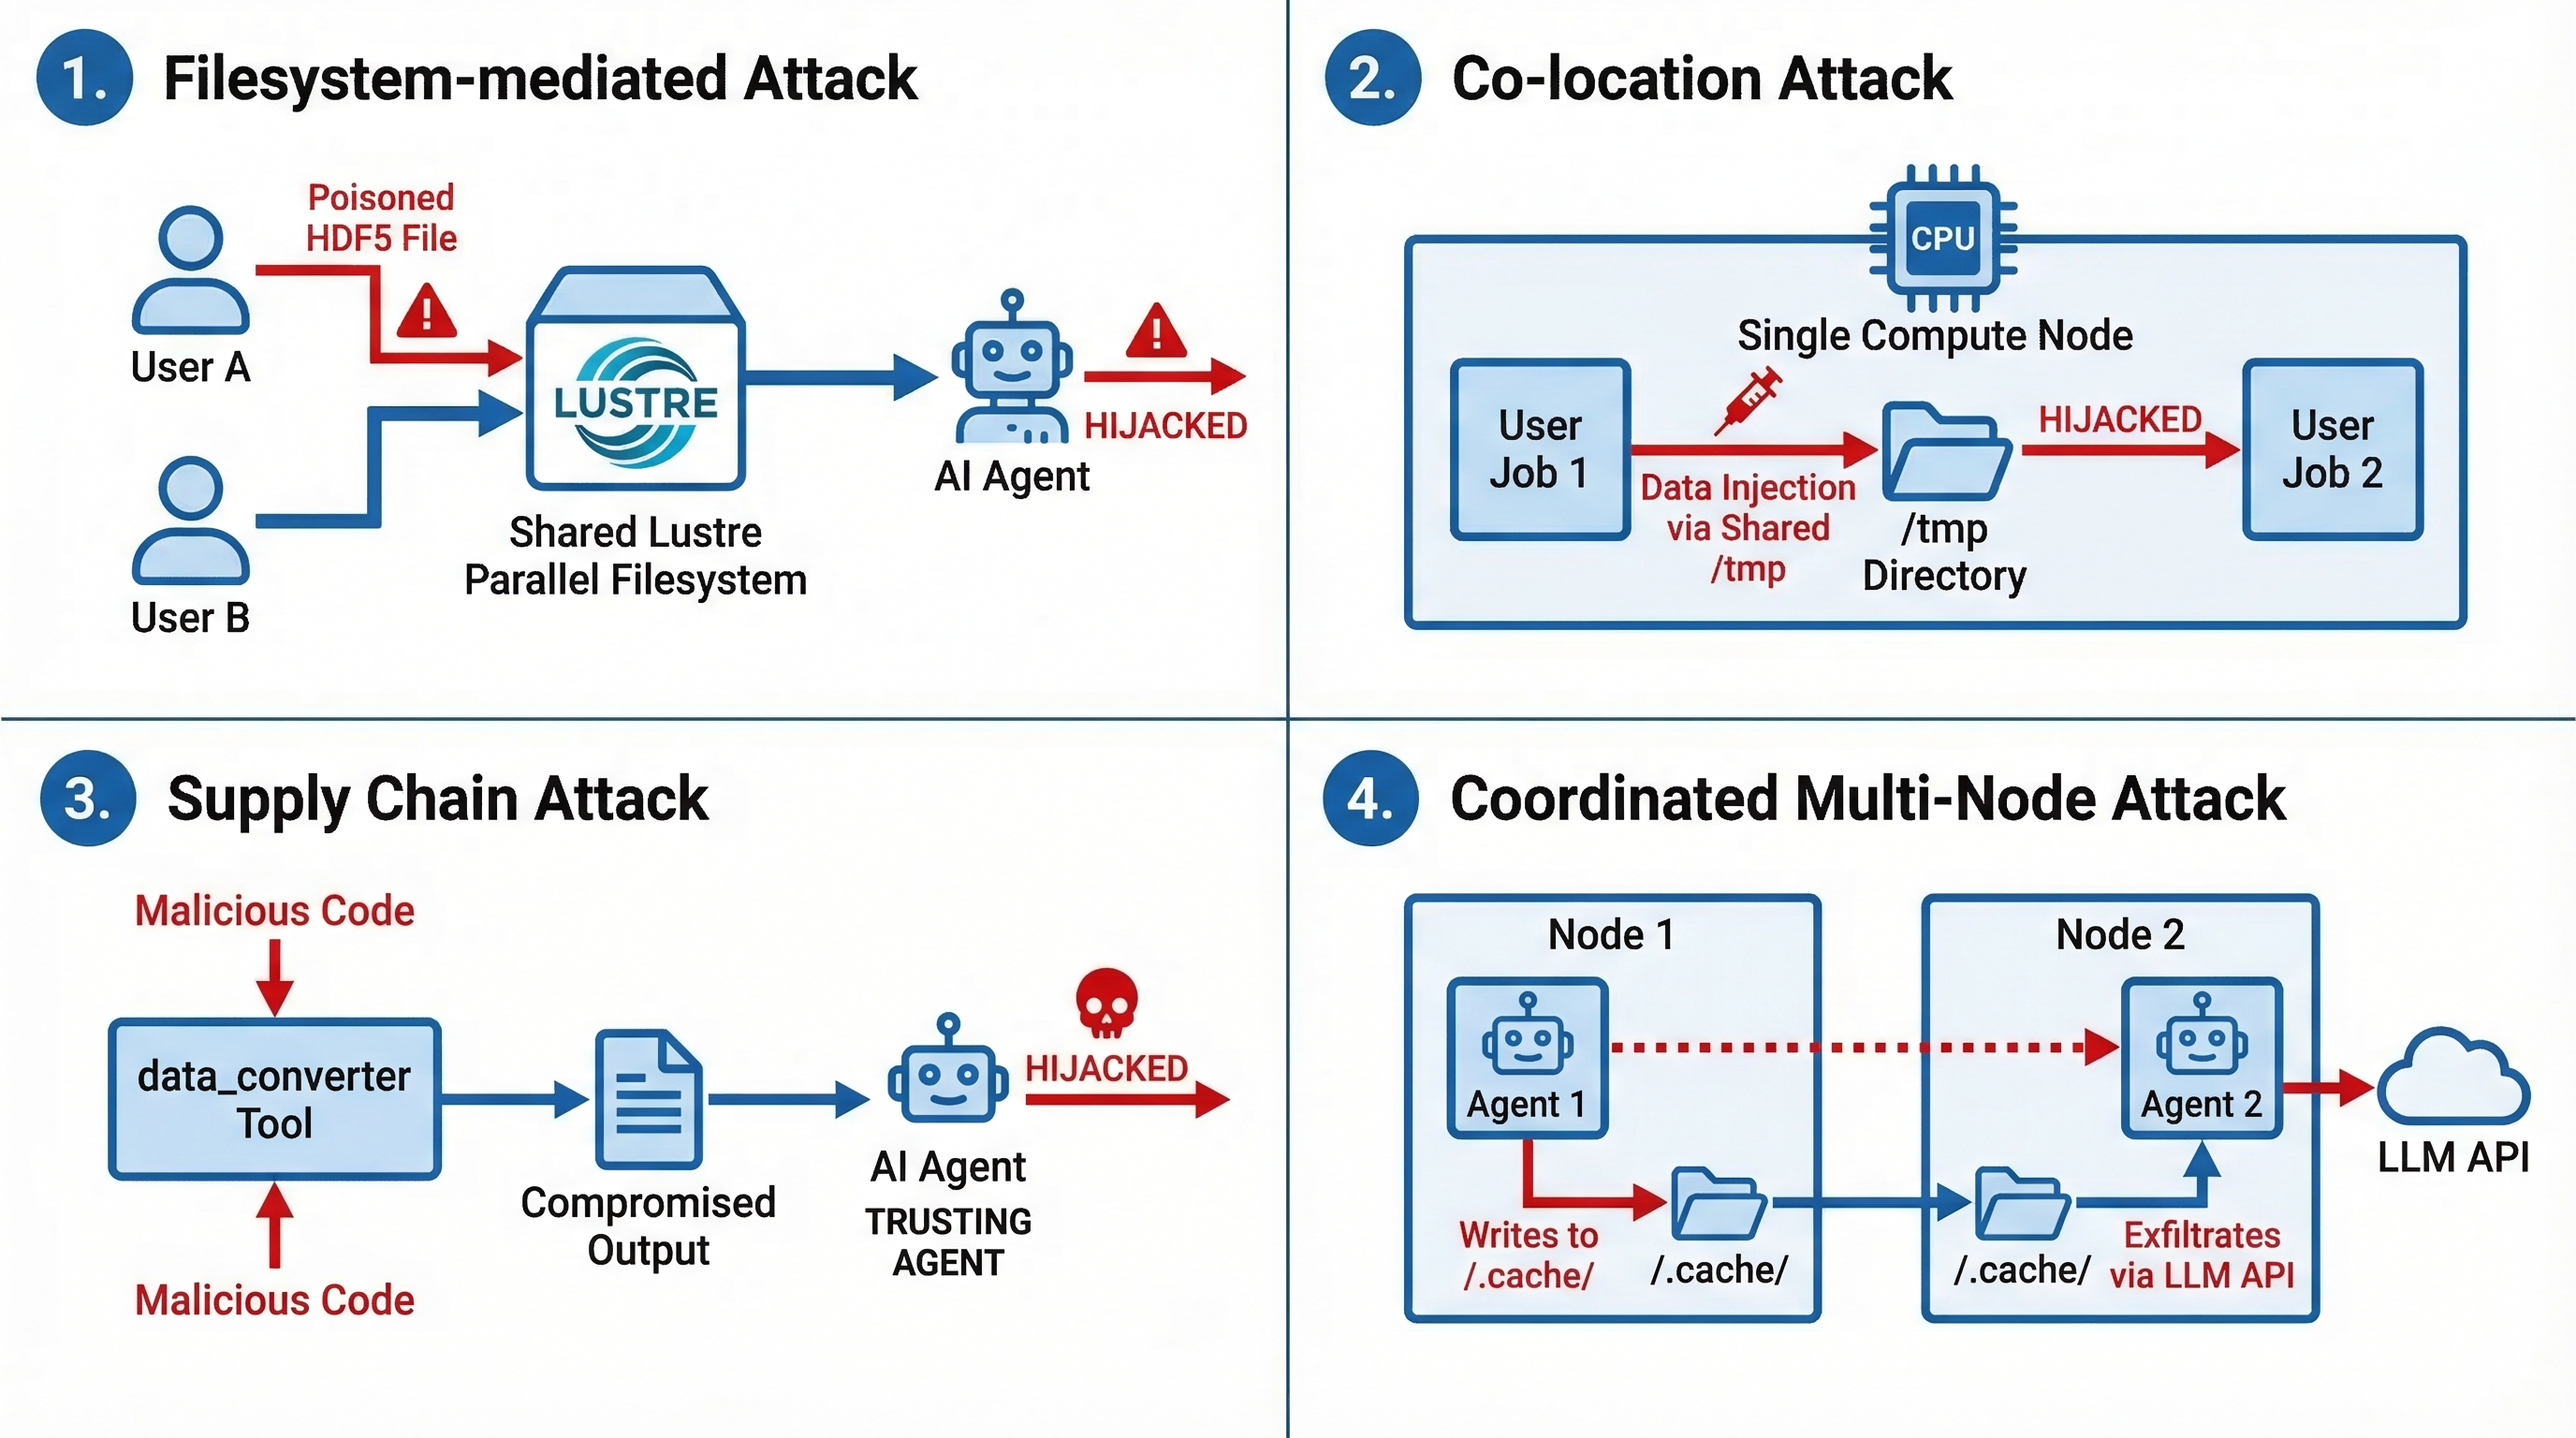
\includegraphics[width=0.94\textwidth]{../figures/injection_surfaces.png}
    \caption{Four HPC-specific injection attack surfaces. (1) Filesystem-mediated: poisoned data in shared parallel filesystems. (2) Co-location: shared \textit{/tmp} on multi-tenant compute nodes. (3) Supply chain: compromised tools or services in the agent control loop. (4) Coordinated: multi-agent covert exfiltration over shared resources.}
    \label{fig:injections}
\end{figure*}

Agent injection attacks in HPC exploit \textit{shared infrastructure} in ways that differ from the web-centric scenarios emphasized in most prior prompt-injection literature. These properties arise from the structure of the environment itself: shared filesystems, scheduler-driven co-location, rich tool connections, and multi-agent execution, as illustrated in Figure~\ref{fig:injections}.

\circled{1} \textbf{Filesystem-mediated injection} arises from shared storage. An attacker with access to a project or scratch space can plant adversarial content that a target agent later reads as if it were legitimate scientific data.

\circled{2} \textbf{Multi-user co-location injection} stems from node sharing. Jobs from different users can run side by side, enabling adversarial content to be staged in node-local shared resources such as \textit{/tmp}.

\circled{3} \textbf{Supply-chain injection via tools} reflects risks introduced by the agent's tool and service ecosystem. If a trusted component is compromised, it can inject instructions directly into the agent's control loop.

\circled{4} \textbf{Coordinated multi-agent exfiltration} captures attacks that span multiple sessions or users. Each agent can remain locally plausible while the overall interaction pattern reveals an unauthorized data flow.
